%%% MCCA stands for "Master-class of the Computer Archaeology"
\documentclass[t,aspectratio=169]{beamer}
\usepackage[utf8]{inputenc}
\usepackage[english,russian]{babel}
\usepackage{amsmath,amsfonts, amsthm,amssymb}
\usepackage{dsfont}
\usepackage{enumitem}
\usepackage{bbm}
\usefonttheme[onlymath]{serif}
\usepackage{graphicx}
\graphicspath{{./images}}
\usepackage{xlop}
\usepackage[absolute,overlay]{textpos}
\textblockorigin{10mm}{10mm} % start everything near the top-left corner
\usepackage{soul}
\newcounter{binst}
\makeatletter
\newcommand{\FormatBinary}[1]{\begingroup%
\setcounter{binst}{0}
\def\SOUL@soeverytoken{%
\stepcounter{binst}%
\ifnum\value{binst}=5\relax%
\setcounter{binst}{1}\,%
\fi%
\the\SOUL@token}%
\so{#1}\endgroup} 
\makeatother
\usepackage{booktabs}

\ExplSyntaxOn

\NewDocumentCommand{\binaryaddition}{mm}
 {
  \kartashuvit_binadd:nn { #1 } { #2 }
 }

\tl_new:N \l__kartashuvit_binadd_a_tl
\tl_new:N \l__kartashuvit_binadd_b_tl
\tl_new:N \l__kartashuvit_binadd_c_tl

\cs_new_protected:Nn \kartashuvit_binadd:nn
 {
  \tl_set:Nx \l__kartashuvit_binadd_c_tl
   {
    \int_to_bin:n { \int_from_bin:n { #1 } + \int_from_bin:n { #2 } }
   }
  % pad the summands with \scan_stop:
  \tl_set:Nx \l__kartashuvit_binadd_a_tl
   {
    \prg_replicate:nn
     { \tl_count:N \l__kartashuvit_binadd_c_tl - \tl_count:n { #1 } }
     { \scan_stop: }
    #1
   }
  \tl_set:Nx \l__kartashuvit_binadd_b_tl
   {
    \prg_replicate:nn
     { \tl_count:N \l__kartashuvit_binadd_c_tl - \tl_count:n { #2 } }
     { \scan_stop: }
    #2
   }
  \group_begin:
  \setlength{\tabcolsep}{3pt}
  \begin{tabular}{@{} c *{ \tl_count:N \l__kartashuvit_binadd_c_tl } { c } }
  \tl_map_function:NN \l__kartashuvit_binadd_a_tl \__kartashuvit_binadd_tab:n \\
  +
  \tl_map_function:NN \l__kartashuvit_binadd_b_tl \__kartashuvit_binadd_tab:n \\
  \midrule
  \tl_map_function:NN \l__kartashuvit_binadd_c_tl \__kartashuvit_binadd_tab:n \\
  \end{tabular}
  \group_end:
 }

\cs_new:Nn \__kartashuvit_binadd_tab:n { & #1 }

\ExplSyntaxOff

% I follow the circuitikz manual
% https://ctan.mirror.norbert-ruehl.de/graphics/pgf/contrib/circuitikz/doc/circuitikzmanual.pdf

\usepackage{circuitikz}
\ctikzset{
    logic ports=ieee,
    logic ports/scale=0.7,
}
\tikzset{sr-ff/.style={flipflop, flipflop def={
    t1=S, t2=CP, t3=R, t4={\ctikztextnot{Q}},
    t6=Q, nd=1}},
}

\usepackage{amsmath}

\usepackage{verbatim}
\usepackage{listings}

\addtobeamertemplate{navigation symbols}{}{%
    \usebeamerfont{footline}%
    \usebeamercolor[fg]{footline}%
    \hspace{1em}%
    \insertframenumber/\inserttotalframenumber
}

\newcommand{\backupbegin}{
   \newcounter{finalframe}
   \setcounter{finalframe}{\value{framenumber}}
}
\newcommand{\backupend}{
   \setcounter{framenumber}{\value{finalframe}}
}
\usepackage{url}

\author{Андрей Рабусов}
\date{Ноябрь 2022}
\title{Археология компьютеров\\
Мастер-класс}

\begin{document}
\begin{frame}
    \frametitle{Содержание}
    \tableofcontents[sectionstyle=show,subsectionstyle=show]
\end{frame}

\section*{Введение}
\begin{frame}
    \frametitle{Компьютеры сейчас и тогда}
    \begin{figure}
        \begin{centering}
            \only<1>{
                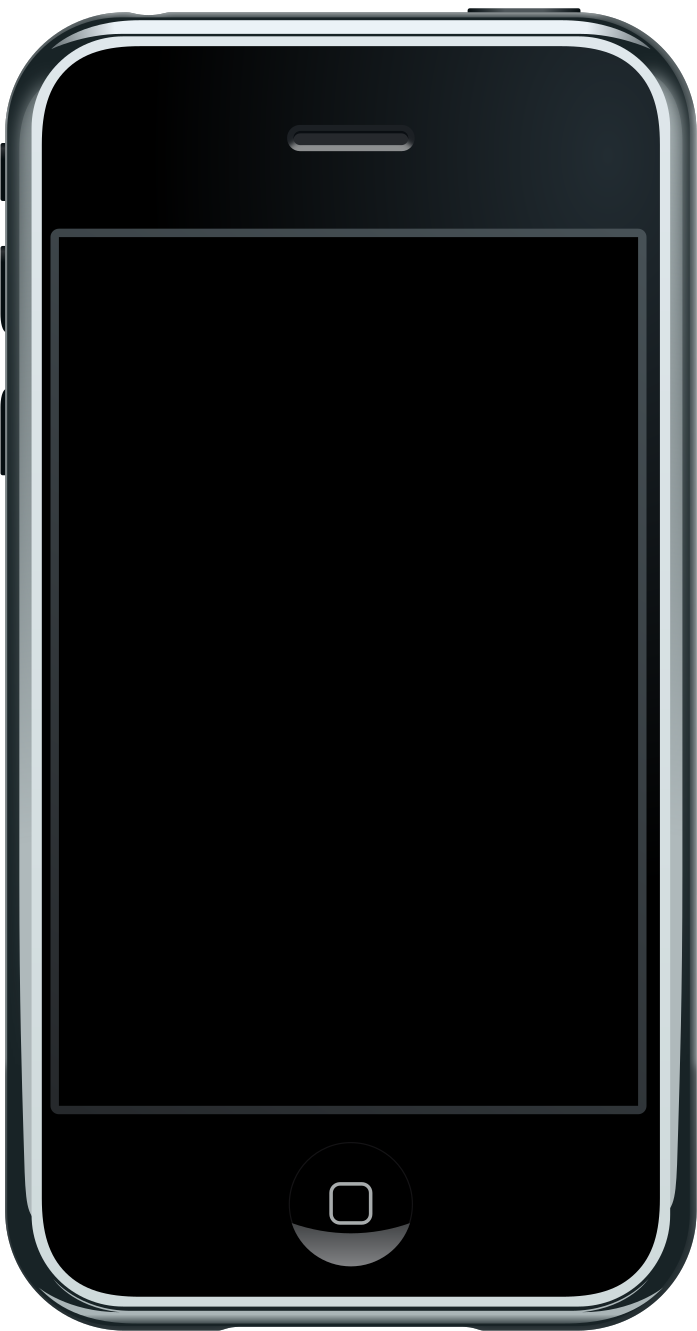
\includegraphics[height=0.7\textheight]{iphone}
                % Credit: https://upload.wikimedia.org/wikipedia/commons/a/ad/IPhone_1st_Gen.svg
                \caption{iPhone, 1st gen.}
            }
            \only<2>{
                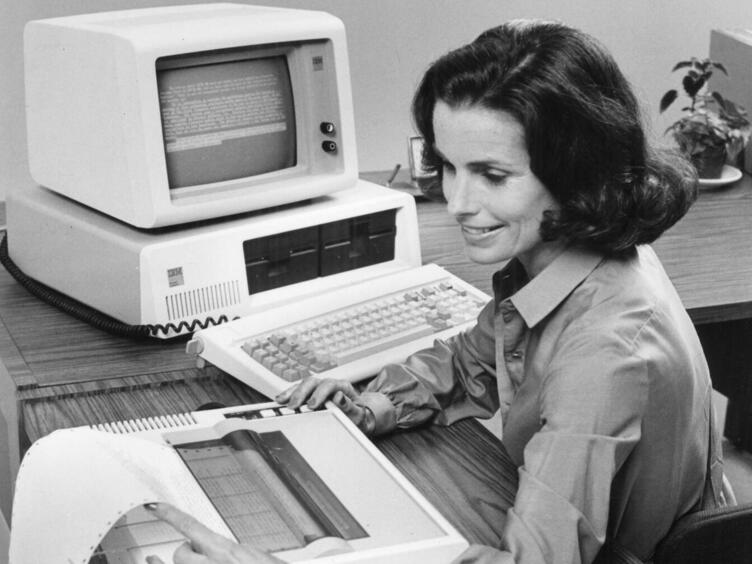
\includegraphics[height=0.7\textheight]{ibm-pc}
                % Credit: https://www.rheinpfalz.de/wirtschaft_artikel,-ein-pc-f%C3%BCr-18-000-dollar-_arid,5239259.html
                \caption{IBM PC}
            }
            \only<3>{
                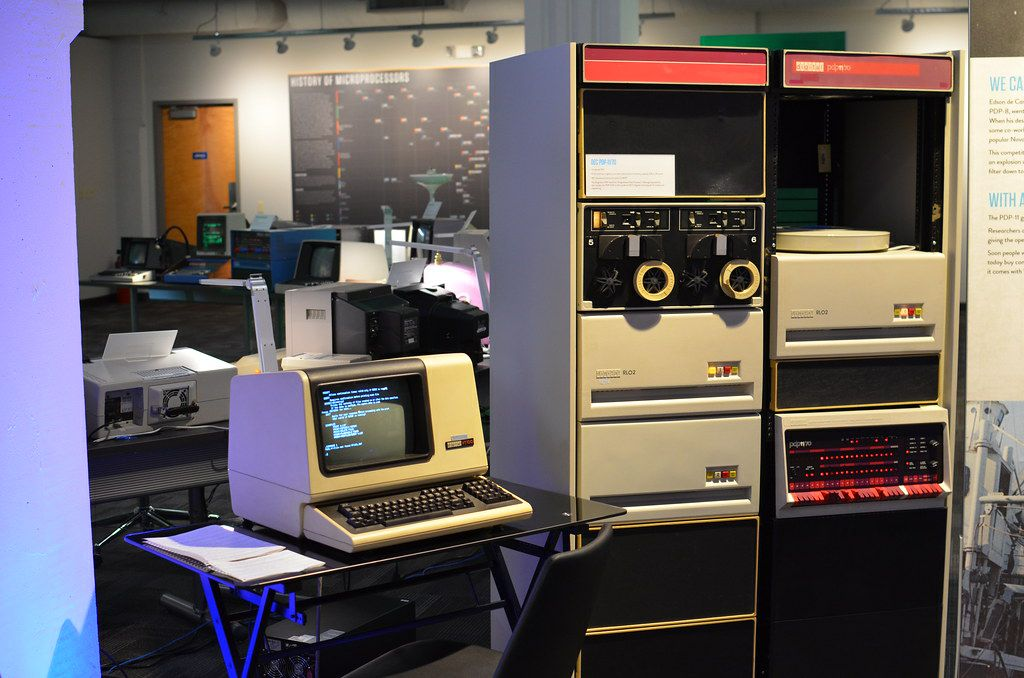
\includegraphics[height=0.7\textheight]{cm-pdp11}
                \caption{PDP-11/70}
            }
            \only<4>{
                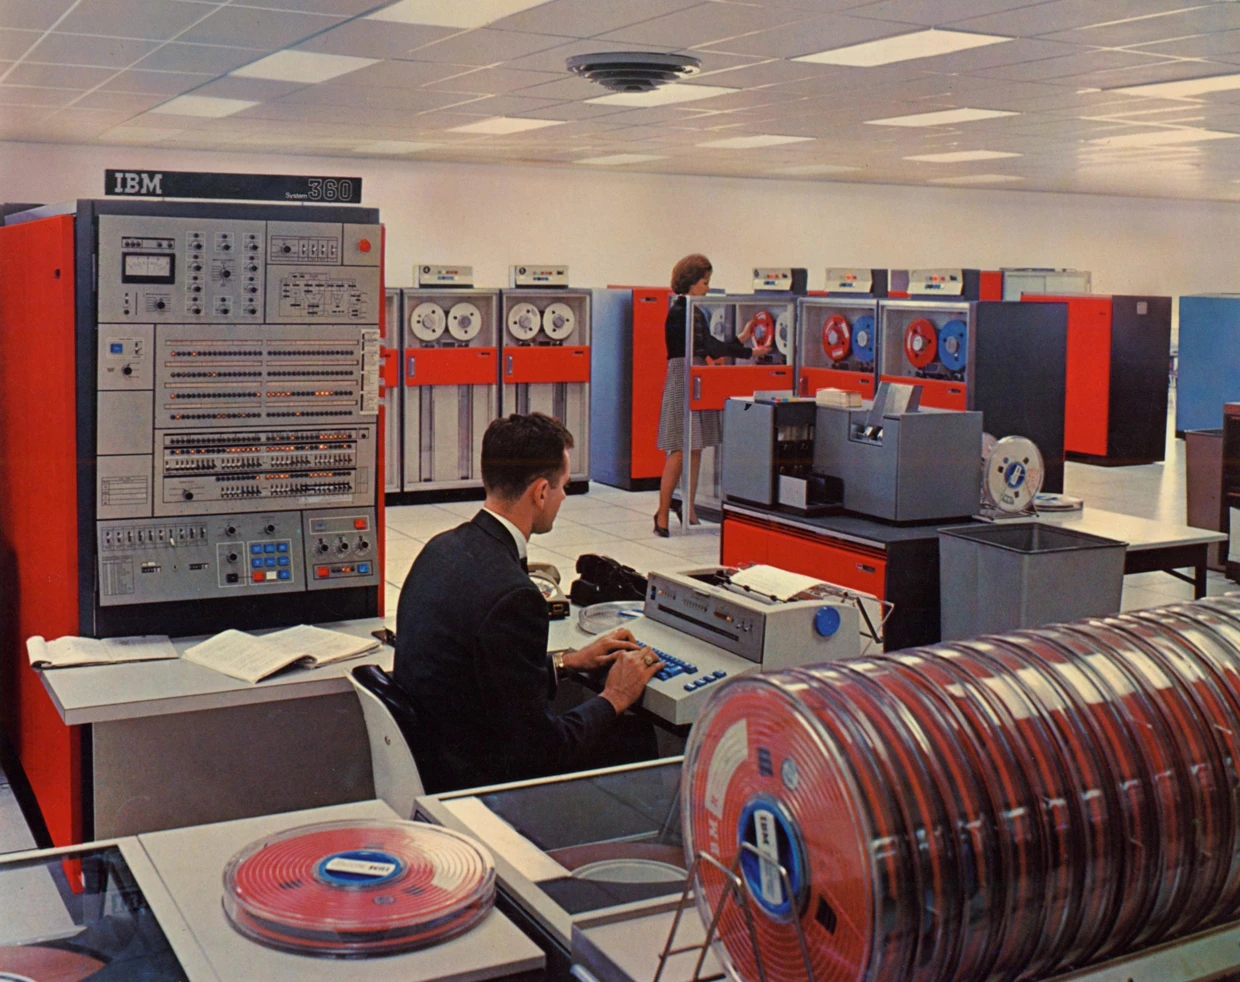
\includegraphics[height=0.7\textheight]{ibm-360}
                % Credit: https://media-cldnry.s-nbcnews.com/image/upload/t_fit-1240w,f_auto,q_auto:best/newscms/2014_19/432091/140509-ibm-360-mn-1120.jpg
                \caption{IBM 360}
            }
            \only<5>{
                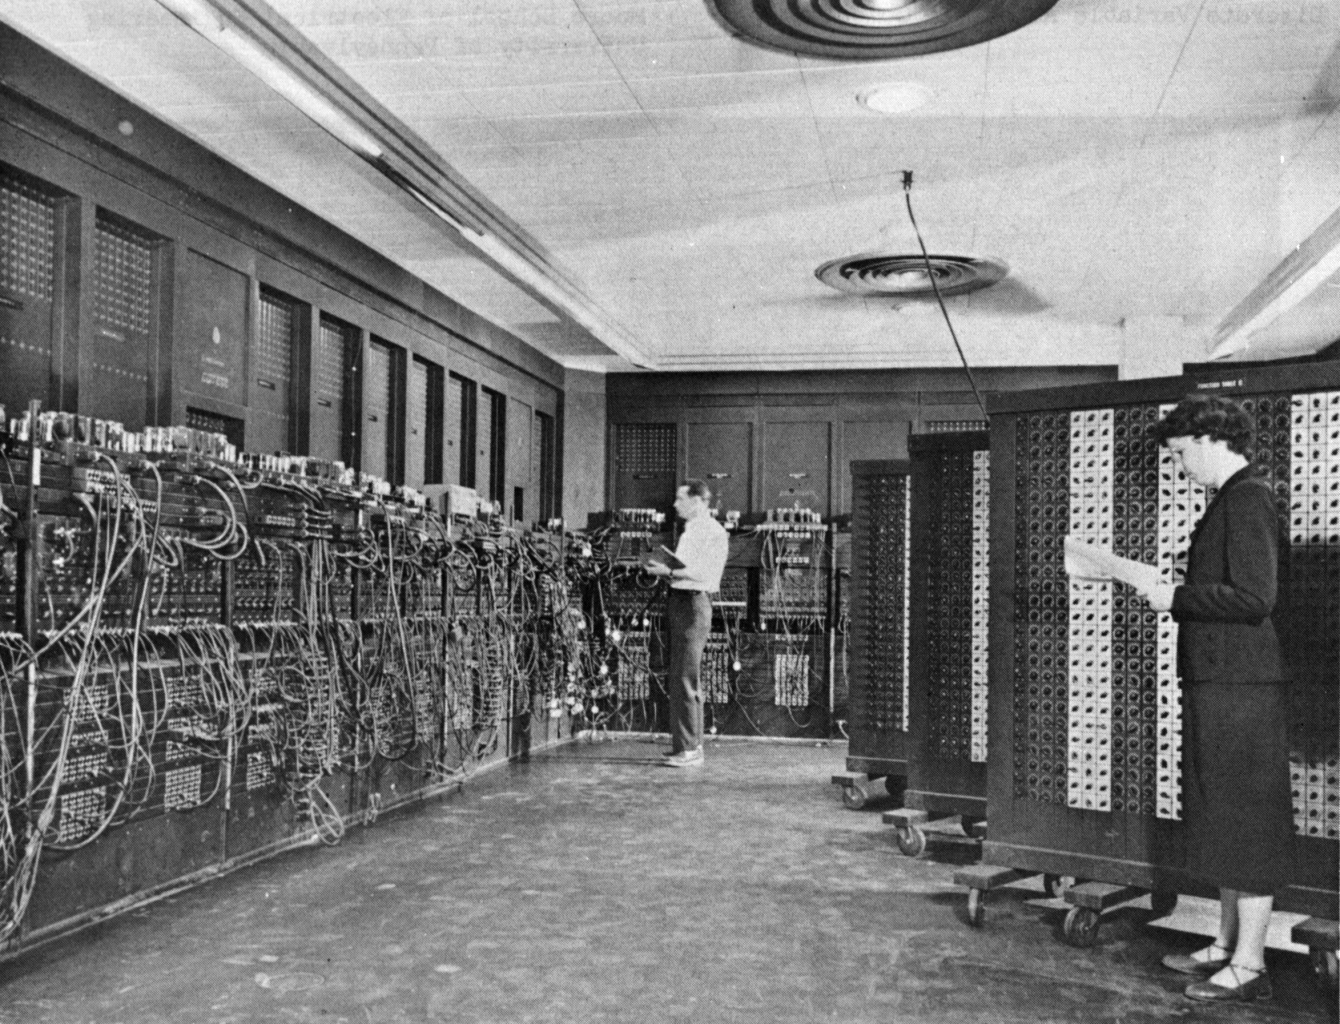
\includegraphics[height=0.7\textheight]{Eniac}
                % Credit: https://upload.wikimedia.org/wikipedia/commons/4/4e/Eniac.jpg
                \caption{Eniac}
            }
        \end{centering}
    \end{figure}

\end{frame}

\section{<<Железо>>}
\begin{frame}
    \frametitle{Двоичные числа}
    \begin{equation*}
        \FormatBinary{10110101}_2 =
        1\cdot 2^0 +
        0 \cdot 2^1 +
        1 \cdot 2^2 +
        0 \cdot 2^3 + 
        1 \cdot 2^4 + 
        0 \cdot 2^5 + 
        1 \cdot 2^6 + 
        1 \cdot 2^7 = 181
    \end{equation*}
    \par\vspace{0.25cm}
    \begin{minipage}{0.75\textwidth}
        Сложение чисел в обычной (десятеричной) системе:
    \end{minipage}
    \begin{minipage}{0.24\textwidth}
        \opadd{384}{56}\qquad\par\vspace{0.5cm}
    \end{minipage}
    \begin{minipage}{0.75\textwidth}
        Сложение чисел в двоичной системе:
    \end{minipage}
    \begin{minipage}{0.24\textwidth}
        \binaryaddition{1010}{1001}\qquad\par
    \end{minipage}
\end{frame}

\begin{frame}
    \frametitle{Логические операции}
    \begin{columns}
        \begin{column}{0.49\textwidth}
            \begin{minipage}{0.69\textwidth}
                \begin{equation*}
                    \begin{array}{c|c}
                        \toprule
                        x & \mathrm{not}\;x\\
                        \hline
                        0 & 1 \\
                        1 & 0 \\
                        \bottomrule
                    \end{array}
                \end{equation*}
            \end{minipage}
            \begin{minipage}{0.19\textwidth}
                \begin{tikzpicture}[scale=0.1]
                    \node[ieeestd not port] (not1) at (0,0) {};
                \end{tikzpicture}
            \end{minipage}
            \par\vspace{1.0cm}
            \begin{minipage}{0.69\textwidth}
                \begin{equation*}
                    \begin{array}{c|c|c}
                        \toprule
                        x & y & x\;\mathrm{and}\;y \\
                        \hline
                        0 & 0 & 0 \\
                        1 & 0 & 0 \\
                        0 & 1 & 0 \\
                        1 & 1 & 1 \\
                        \bottomrule
                    \end{array}
                \end{equation*}
            \end{minipage}
            \begin{minipage}{0.19\textwidth}
                \begin{tikzpicture}[scale=0.1]
                    \node[ieeestd and port] (and1) at (0,0) {};
                \end{tikzpicture}
            \end{minipage}
        \end{column}

        \begin{column}{0.49\textwidth}
            \begin{minipage}{0.69\textwidth}
                \begin{equation*}
                    \begin{array}{c|c|c}
                        \toprule
                        x & y & x\;\mathrm{or}\;y \\
                        \hline
                        0 & 0 & 0 \\
                        1 & 0 & 1 \\
                        0 & 1 & 1 \\
                        1 & 1 & 1 \\
                        \bottomrule
                    \end{array}
                \end{equation*}
            \end{minipage}
            \begin{minipage}{0.19\textwidth}
                \begin{tikzpicture}[scale=0.1]
                    \node[ieeestd or port] (or1) at (0,0) {};
                \end{tikzpicture}
            \end{minipage}
            \par\vspace{1.0cm}
            \begin{minipage}{0.69\textwidth}
                \begin{equation*}
                    \begin{array}{c|c|c}
                        \toprule
                        x & y & x\;\mathrm{xor}\;y \\
                        \hline
                        0 & 0 & 0 \\
                        1 & 0 & 1 \\
                        0 & 1 & 1 \\
                        1 & 1 & 0 \\
                        \bottomrule
                    \end{array}
                \end{equation*}
            \end{minipage}
            \begin{minipage}{0.19\textwidth}
                \begin{tikzpicture}[scale=0.1]
                    \node[ieeestd xor port] (xor1) at (0,0) {};
                \end{tikzpicture}
            \end{minipage}
        \end{column}
    \end{columns}
\end{frame}

\begin{frame}
    \frametitle{Арифметические операции}
\end{frame}

\begin{frame}
    \frametitle{Переключатели: кирпичи в компьютерах}

\end{frame}

\begin{frame}
    \frametitle{Как запоминает компьютер?}
    \begin{columns}
        \begin{column}{0.49\textwidth}
            %%% Taken from: https://latexdraw.com/draw-sr-flip-flop-with-circuitikz/
            \begin{tikzpicture}[scale=0.5]

                % AND logic gates
                \node[ieeestd and port] (and1) at (0,2) {};
                \node[ieeestd and port] (and2) at (0,-2) {};

                % NOR logic gates
                \draw (and1.out) -- ++(2.5,0) node[ieeestd nor port, anchor=in 1] (nor1) {};
                \draw (and2.out) -- ++(2.5,0) node[ieeestd nor port, anchor=in 2] (nor2) {};

                \draw (nor1.in 2) -| ++ (-0.2,-0.85) -- ++(3,-1.5) coordinate(a) |- (nor2.out);
                \draw (nor2.in 1) -| ++ (-0.2,0.85) -- ++(3,1.5) |- (nor1.out);

                % Labels
                \draw (and1.in 1) -- ++(-0.75,0) node[left]{R};
                \draw (and2.in 2) -- ++(-0.75,0) node[left]{S};
                \draw (and1.in 2) -- (and2.in 1)node[midway](clk){};
                \draw (clk.center) -- ++(-0.75,0) node[left]{Clk};

                \draw (nor1.out -| a) -- ++(0.75,0) node[right]{Q(t)};
                \draw (nor2.out -| a) -- ++(0.75,0) node[right]{Q(t)$^{'}$};

            \end{tikzpicture}
        \end{column}
        \begin{column}{0.49\textwidth}
            \begin{circuitikz}[]
                \draw (0,0) node[sr-ff](FF){} (FF.bup)
                node[above]{SR-FF};
                \draw (FF.pin 1) -- ++(-1,0) node[and port,
                anchor=out](AND1){}
                (FF.pin 3) -- ++(-1,0) node[and port,
                anchor=out](AND2){};
            \end{circuitikz}
        \end{column}
    \end{columns}
\end{frame}

\section{Взаимодействие человек--машина}
\begin{frame}
    \frametitle{Перфокарты}
\end{frame}

\begin{frame}
    \frametitle{Перфоленты}
\end{frame}

\begin{frame}
    \frametitle{Телетайп}
\end{frame}

\begin{frame}
    \frametitle{Терминал}
\end{frame}

\section{Программы}
\begin{frame}
    \frametitle{Игры: Space Travel}
\end{frame}

\begin{frame}
    \frametitle{Как обмануть начальство?}
\end{frame}

\begin{frame}
    \frametitle{Что такое программа?}
\end{frame}

\begin{frame}
    \frametitle{UNIX room}
\end{frame}

\begin{frame}
    \frametitle{Командная строка}
\end{frame}

\begin{frame}
    \frametitle{Текстовый редактор}
\end{frame}

\end{document}
